\chapter{Implementacja baz danych w środowisku MySQL}

By zaimplementować kilka rozproszonych węzłów bazy danych posłużono się programem docker, który określany jest jako narzędzie pozwalające umieścić program oraz jego zależności w lekkim, przenośnym, wirtualnym kontenerze, który można uruchomić na prawie każdym serwerze z systemem. 

\section{Konfiguracja kontenerów z środowiskiem MySQL 5.7 i phpMyAdmin}
W celu instalacji programu \textit{Docker} w systemie Ubuntu16.04 posłużono się poniższymi komendami.

\lssetdef
\lstinputlisting[captionpos=b,caption={Instalacja programu docker w systemie ubuntu 16.04},label={lst:docker},basicstyle={\footnotesize\ttfamily}]{rozdzial04/docker.txt}

Następnie zostały pobrane obrazy \textit{MySQL 5.7} oraz \textit{phpmyadmin}

\lssetdef
\lstinputlisting[captionpos=b,caption={Pobranie obrazów z repozytorium},label={lst:images},basicstyle={\footnotesize\ttfamily}]{rozdzial04/images.txt}

Kolejnym krokiem było zapewnienie by można było uruchomić kilka identycznych kontenerów jednocześnie. W tym celu skorzystano z narzędzia Docker Compose. By je zainstalować użyto poniższe komendy.

\lssetdef
\lstinputlisting[captionpos=b,caption={Instalacja narzędzia Docker Compose},label={lst:compose1},basicstyle={\footnotesize\ttfamily}]{rozdzial04/docker-compose.txt}

W poniższym listingu zamieszczona została zawartość pliku docker-compose.yml. Narzędzie dzięki temu plikowi generuje pięć kontenerów z MySQL 5.7 oraz pięć instancji narzędzia phpmyadmin. Czyli w sumie dziesięć serwisów. Każdy został przekierowany na osobny port. Przez co z łatwością można operować tymi serwisami z poziomu przeglądarki internetowej poprzez localhost.

\lssetdef
\lstinputlisting[captionpos=b,caption={Utworzony plik docker-compose.yml},label={lst:compose1},basicstyle={\footnotesize\ttfamily}]{rozdzial04/docker-compose.yml}

Generowanie serwisów z pliku odbywa się poprzez wydanie komendy \textit{docker-compose up} znajdując się w katalogu z plikiem docker-compose.uml.

\section{Konfiguracja mechanizmów replikacji master-slave}
By móc skorzystać z replikacji master-slave każdy węzeł rozproszonej bazy danych musi utworzoną bazę. Dodatkowo trzeba dla każdego węzła zmodyfikować plik konfiguracyjny my.cnf serwisu z MySQl. W pliku tym należy nadać każdemu węzłowi unikalny parametr server-id. Dodatkowo w węźle master w zakładce [mysqld] należy dodać linie z listingu \ref{lst:my.cnf}, a następnie w phpmyadmin  wcisnąć przycisk "GO"

\lssetdef
\lstinputlisting[captionpos=b,caption={Konfiguracja serwera master- modyfikacja pliku my.cnf},label={lst:my.cnf},basicstyle={\footnotesize\ttfamily}]{rozdzial04/mycnf.txt}

\begin{figure} [H]
	\centering
	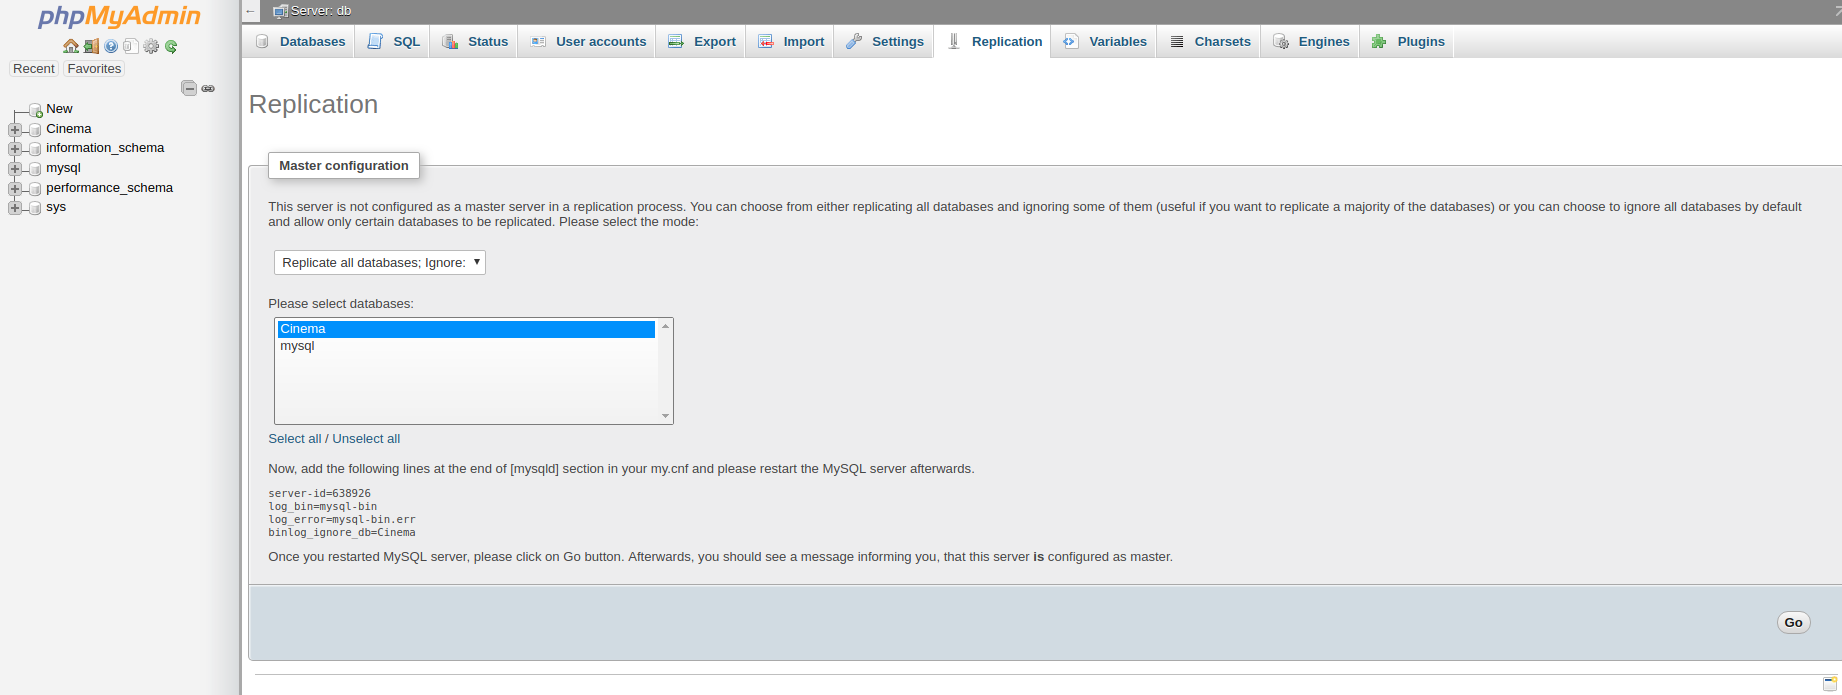
\includegraphics[width=1\linewidth]{rozdzial04/4.png}
	\caption{Konfiguracja serwera master w phpmyadmin}
	\label{fig:phpmyadmin2}
\end{figure}


By ustawić serwer jako slave, należy podać login i hasło do konta w węźle master, podać adres hosta oraz port, a następnie wcisnąć przycisk "GO".

\begin{figure} [H]
	\centering
	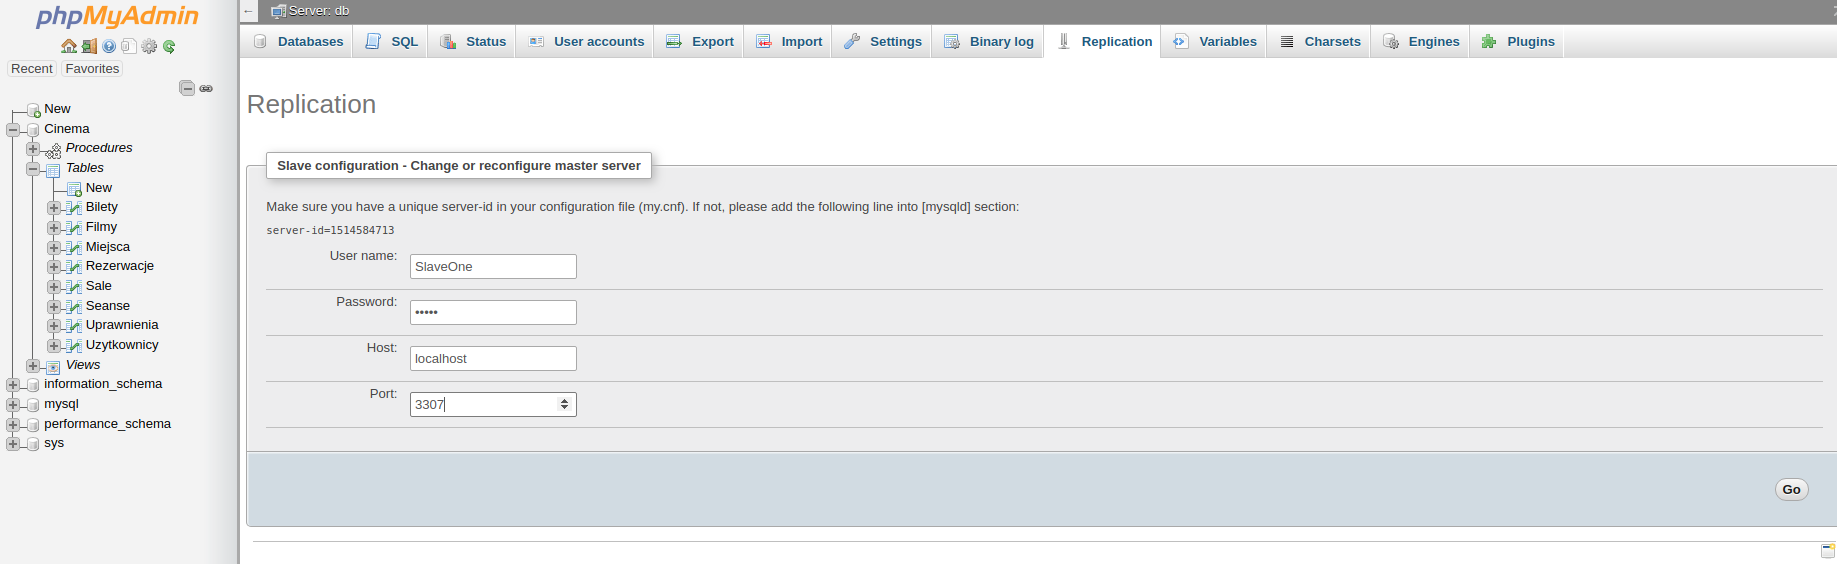
\includegraphics[width=1\linewidth]{rozdzial04/3.png}
	\caption{Konfiguracja serwera slave w phpmyadmin}
	\label{fig:phpmyadmin1}
\end{figure}

By dodać opóźnienie do węzła slave można z poziomu panelu phpmyadmin w zakładce SQL wydać komendę:

\lssetdef
\lstinputlisting[captionpos=b,caption={Konfiguracja opóźnienia dla węzła slave},label={lst:slave},basicstyle={\footnotesize\ttfamily}]{rozdzial04/slave.txt}

Dla takich danych opóźnienie wyniesie 120 sekund.

\section{Realizacja bazy danych}

\subsection{Tabele}

Tabele generowano za pomocą skryptów MySQL.

\begin{itemize}
	\item zdefiniowano klucze główne;
	\item zdefiniowano klucze obce;
	\item dodano ograniczenia jeżeli jakiś element nie może być pusty;
	\item tam gdzie to konieczne (login użytkownika ,nazwa sali i nazwa uprawnień) dodano ograniczenia, aby dane te były unikalne w swoich tabelach;
	\item sprawdzanie czy podana liczba należy do przedziału wykorzystując słowo kluczowe \textit{CHECK} (pojemność sali musi się znajdować w przedziale od 20 do 450 miejsc);
	\item zabezpieczenie przed nadpisywaniem już wcześniej utworzonych tabel \textit{IF NOT EXISTS}.
\end{itemize}

\begin{figure} [H]
	\centering
	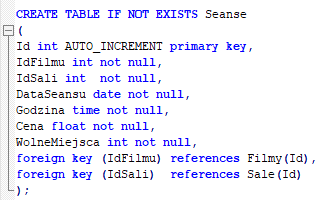
\includegraphics[width=0.6\linewidth]{rozdzial04/T_Seanse.png}
	\caption{Generowanie tabeli seansów}
	\label{fig:t_seanse}
\end{figure}

\begin{figure} [H]
	\centering
	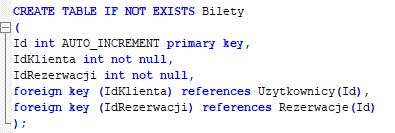
\includegraphics[width=0.6\linewidth]{rozdzial04/T_Bilety.png}
	\caption{Generowanie tabeli biletów - przykład użycia klucza głównego, kluczy obcych i ograniczenia "not null"}
	\label{fig:t_bilety}
\end{figure}

\begin{figure} [H]
	\centering
	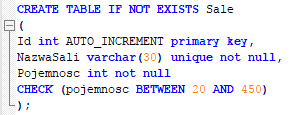
\includegraphics[width=0.5\linewidth]{rozdzial04/T_Sale.png}
	\caption{Generowanie tabeli sal - przykład użycia CHECK}
	\label{fig:t_sale}
\end{figure}

\subsection{Widoki}

\textbf{Utworzono trzy widoki:}

\begin{figure} [H]
	\centering
	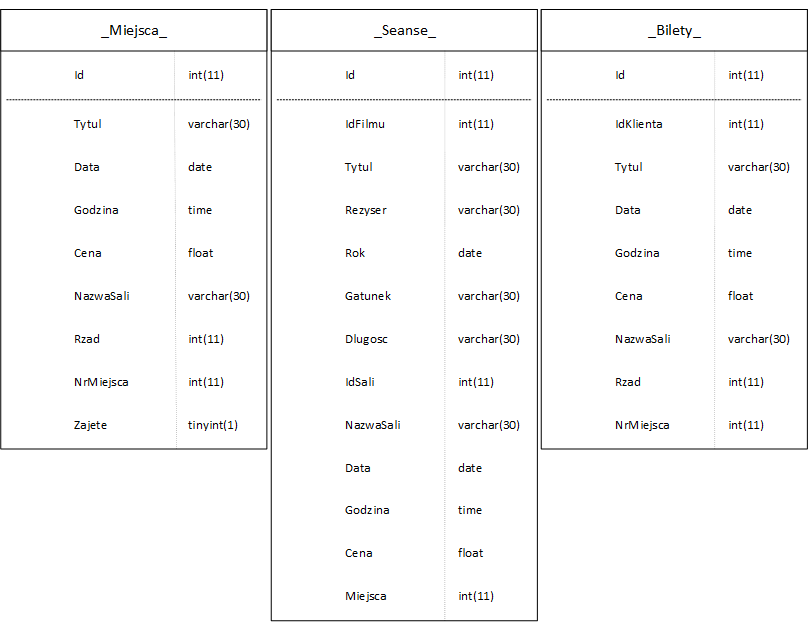
\includegraphics[width=0.8\linewidth]{rozdzial04/widoki.png}
	\caption{Wygenerowane widoki}
	\label{fig:views}
\end{figure}

\begin{itemize}
	\item \_Seanse\_ - rozszerza tabelę \textit{Seanse} o dodatkowe informacje o filmie, którego dotyczy seans i sali, na której seans zostanie wyświetlony;
	\item \_Miejsca\_ - rozszerza tabelę \textit{Rezerwacje} o informacje takie jak nazwa sali, rząd i numer miejsca.
	\item \_Bilety\_ - rozszerza tabelę \textit{Bilety} o informacje takie jak tytuł filmu, data, cena, nazwa sali, rząd oraz numer miejsca
\end{itemize}

\begin{figure} [H]
	\centering
	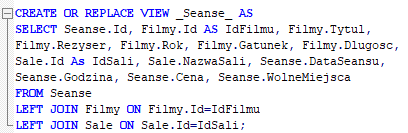
\includegraphics[width=0.6\linewidth]{rozdzial04/V_Seanse_.png}
	\caption{Generowanie widoku seansów}
	\label{fig:v_seanse}
\end{figure}

\begin{figure} [H]
	\centering
	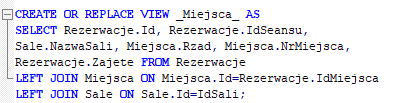
\includegraphics[width=0.6\linewidth]{rozdzial04/V_Miejsca_.png}
	\caption{Generowanie widoku Miejsc}
	\label{fig:v_miejsca}
\end{figure}

\subsection{Procedury}

Rysunek \ref{fig:procedury} przedstawia wszystkie procedury jakie zostały zaimplementowane. Natomiast na rysunku \ref{fig:p_DodajSeans} pokazana została jedna przykładowa procedura, która dodając seans dodaje również pulę miejsc równą pojemności sali, w której odbędzie się seans do tabeli \textit{Rezerwacje}.
\begin{figure} [H]
	\centering
	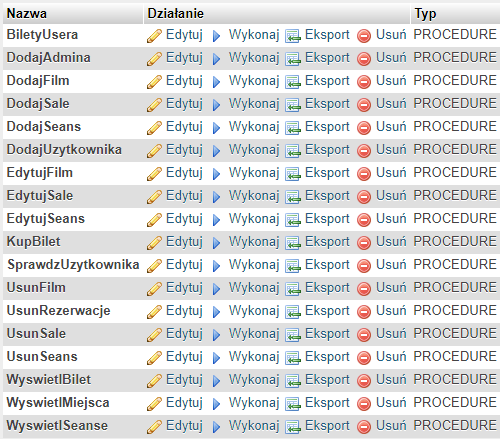
\includegraphics[width=0.7\linewidth]{rozdzial04/Procedury.png}
	\caption{Przykładowa procedura}
	\label{fig:procedury}
\end{figure}

\textbf{Opisy procedur:}
\begin{itemize}
	\item BiletyUsera - wyświetla wszystkie bilety które zostały zakupione przez konkretnego użytkownika;
	\item DodajAdmina - procedura pozwala na dodanie nowego użytkownika o uprawnieniach administratora;
	\item DodajFilm - pozwala na dodanie nowego filmu do filmoteki kina;
	\item DodajSale - pozwala dodać do bazy danych nowej sali kinowej;
	\item DodajSeans - umożliwia dodanie nowego seansu do oferty kina;
	\item DodajUzytkownika - procedura pozwala na dodanie nowego użytkownika o standardowych prawach zwykłego użytkownika;
	\item EdytujFilm - pozwala na zmienienie wszystkich informacji o filmie dostępnych w bazie;
	\item EdytujSale - pozwala na zmianę nazwy sali;
	\item EdytujSeans - pozwala modyfikować datę godzinę i cenę seansu;
	\item KupBilet - tworzy nowy rekord w tabeli Bilety, przypisuje go do konkretnego użytownika, oraz zmienia ilość wolnych miejsc na seansie, a w tabeli Rezerwacje oznacza miejsce jako zajęte;
	\item SprawdzUzytkownika - sprawdza czy użytkownik o podanym loginie i haśle istnieje w systemie;
	\item UsunFilm - usuwa film z filmoteki kina;
	\item UsunRezerwacje - usuwa wszystkie bilet, anuluje transakcję użytkownika, przywraca miejsce jako niezarezerwowane;
	\item UsunSale - usuwa sale i miejsca przypisane do sali, anuluje wszystkie seanse, które miały odbyć się na danej sali, i anuluje wszystkie bilety na te seanse;
	\item UsunSeans - anuluje seans i wszystkie bilety i rezerwacje na niego;
	\item WyswietlBilet - wyświetla informacje o bilecie o podanym id;
	\item WyswietlMiejsca - pokazuje wszystkie wolne miejsca na konkretny seans, korzystając z widoku \_Miejsca\_;
	\item WyswietlSeanse - wyświetla rozszerzone informacje o seansach z podanym filmem, korzystając z widoku \_Seanse\_.
\end{itemize}

\begin{figure} [H]
	\centering
	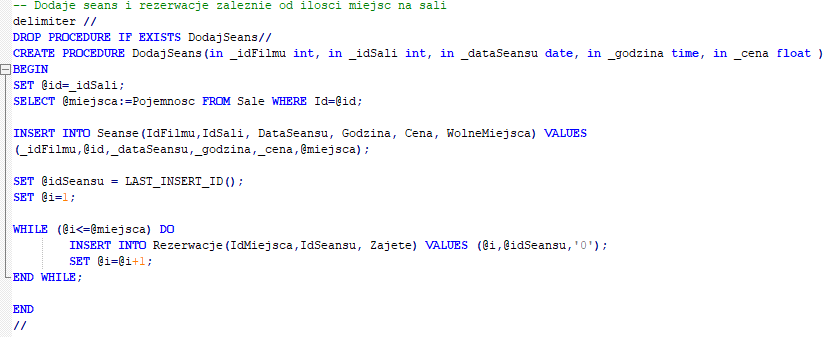
\includegraphics[width=1\linewidth]{rozdzial04/P_DodajSeans.png}
	\caption{Przykładowa procedura}
	\label{fig:p_DodajSeans}
\end{figure}